% Double Arrows a la Chef
% Author: Dominik Haumann
\documentclass{standalone}
\usepackage{tikz}
\usetikzlibrary{arrows, decorations.markings}

% for double arrows a la chef
% adapt line thickness and line width, if needed
\tikzstyle{vecArrow} = [thick, decoration={markings,mark=at position
   1 with {\arrow[semithick]{open triangle 60}}},
   double distance=1.4pt, shorten >= 5.5pt,
   preaction = {decorate},
   postaction = {draw,line width=1.4pt, white,shorten >= 4.5pt}]
\tikzstyle{innerWhite} = [semithick, white,line width=1.4pt, shorten >= 4.5pt]

\begin{document}

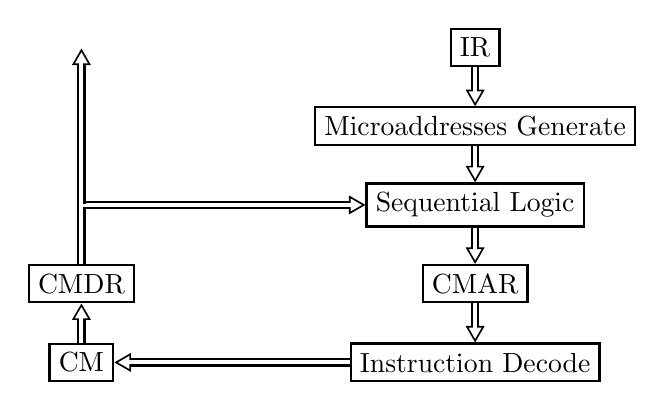
\begin{tikzpicture}[thick]
  \node[draw,rectangle] (h) {IR};
  \node[draw,rectangle,below of=h] (a) {Microaddresses Generate};
  \node[draw,rectangle,below of=a] (b) {Sequential Logic};
  \node[draw,rectangle,below of=b] (c) {CMAR};
	\node[draw,rectangle,below of=c] (d) {Instruction Decode};
\node[inner sep=0,minimum size=0,left of=d] (k) {}; % invisible node
\node[inner sep=0,minimum size=0,left of=k] (l) {}; % invisible node
\node[inner sep=0,minimum size=0,left of=l] (m) {}; % invisible node
\node[inner sep=0,minimum size=0,left of=m] (12) {}; % invisible node
  \node[draw,rectangle,left of=12] (e) {CM};
  \node[draw,rectangle,above of=e] (f) {CMDR};
\node[inner sep=0,minimum size=0,above of= f] (13) {}; % invisible node
\node[inner sep=0,minimum size=0,above of= 13] (14) {}; % invisible node

\node[inner sep=0,minimum size=0,above of= 14] (15) {}; % invisible node
  % 1st pass: draw arrows
  \draw[vecArrow] (h) to (a);
  \draw[vecArrow] (a) to (b);
  \draw[vecArrow] (b) to (c);
  \draw[vecArrow] (c) to (d);
  \draw[vecArrow] (d) to (e);
  \draw[vecArrow] (e) to (f);
  \draw[vecArrow] (f) |- (b);
  \draw[vecArrow] (13) to (15);


  % 2nd pass: copy all from 1st pass, and replace vecArrow with innerWhite
  \draw[innerWhite] (a) to (b);
  %\draw[innerWhite] (b) |- (c);

  % Note: If you have no branches, the 2nd pass is not needed
\end{tikzpicture}

\end{document}